In this chapter, we study and implement numerical methods for solving ODEs(Ordinary differential equations) and PDE (Partial differential equations). In section 2.1-2.3 we study the Two Point Boundary Value problem using the Runge-Kutta method. Next, in section 2.4 we study finite difference methods to treat PDE as numerical simulations given an initial condition to finally apply our model's boundary conditions \ref{eq:boundary-condition-flux} in section 2.5.
\section{Runge-Kutta Method}
\label{sec:run_kut}

The Runge-Kutta Method is used to determine the numerical value of a system of differential equations to which we know the boundary conditions. Let 

$$\vec{y}' = \vec{F}(x, \vec{y})$$
$$\vec{y}(x_0) = \vec{y}_0$$

be the system of equations we want to solve with the method. We approximate the derivative by

$$\frac{\vec{y}(x+h)-\vec{y}(x)}{h} = \vec{F}(x + h, \vec{y}+\vec{y}(x+h))$$

We want to approximate the left hand side with a series expansion to arbitrary order in $h$. We thus obtain an expression for $y(x+h)$,

$$\vec{y}(x+h)=\vec{y}(x)+ h\vec{F}(x + h, \vec{y}+\vec{y}(x+h)).$$

In this work we use the Runge-Kutta of fifth order in the integration step $h$. The expression for the increment at this order of precision is

$$\vec{y}_5(x+h) = \vec{y}(x) + \sum_{i=0}^{6} C_{i} K_i,$$

and

$$K_0 = hF(x,y),$$
$$K_i = hF(x+A_ih,y+\sum_{i=0}^{i-1} B_{ij} K_j)$$

where $i = 1,2,3, .. , 6 $.

We also need the fourth order Runge-Kutta method in order to obtain the error in the integration. This is given by

$$\vec{y}_4(x+h) = \vec{y}(x) + \sum_{i=0}^{6} D_{i} K_i,$$

The error is given by 

\begin{eqnarray}
\vec{E}(h) = \vec{y}_5(x+h) - \vec{y}_4(x+h).
\end{eqnarray}

Of this expression, we can take the root mean square of the components of $\vec{E}(h)$,

\begin{equation}
e(h) = \sqrt{\frac{1}{n}\sum_{i=0}^{n-1}E_i^2(h)}
\end{equation}

This way we obtain a scalar measure of the error.

If $h_1$ and $h_2$ are two consecutive steps in the integration of the differential equation, then it can be shown that

\begin{equation}
\frac{e(h_1)}{e(h_2)} \approx \qty{\frac{h_1}{h_2}}^5
\label{eq:error}
\end{equation}

We don't know what the error of the next step will be, but we can define a tolerance $\epsilon>0$ such that the error of the next step is at most $\epsilon$. Thus, the following step can be computed from Eq. \ref{eq:error} by letting $e(h_2) = \epsilon$

\begin{equation}
h_2= h_1\qty{\frac{\epsilon}{e(h_1)}}^{1/5}
\end{equation}

This method is good for our purposes since the curves we are trying to analyze are flat at the beginning but have sharp slopes towards the interface as will be seen in Chapter 3.

\section{The Shooting Method}
\label{sec:shooting-method}
The method described in section \ref{sec:run_kut} can solve the system of equations if the boundary conditions are all known at a given value of $x = x_0$. Nevertheless, as it can be seen from \ref{eq:two-point-boundary-conditon} through \ref{eq:two-point-boundary-conditon2},
that we have boundary conditions at $x=0$ (the interface) and at $x=\delta$ the bulk solution (see Fig. \ref{fig:geometry}). This is a complication which can be overcome by using the shooting method. The idea is to transform the problem with boundary conditions 

\begin{align}
\label{eq:two-point-boundary-conditon}
	C_+(\delta) = C_-(\delta) = C_b,\\
	\phi(\delta) = 0,\\
	\label{eq:two-point-boundary-conditon2}
	\phi(0) = V_0,
\end{align}


into the problem


\begin{align}
\label{eq:one-point-boundary-conditon}
	C_+(\delta) = C_-(\delta) = C_b,\\
	\phi(\delta) = 0,\\
	E(\delta) = u, 
\end{align}



where $u$ is a constant yet to be determined. To determine $u$, we define a residual function

$$r(u) = \phi(0)-V_0.$$

which is zero when the value of $\phi(0)$ (given an appropriate u) is the original boundary condition. Therefore, the two-point boundary problem is transformed into a  root finding problem. First, we need to find two values of $u$, $u_1$ and $u_2$ such that $r(u_1) < 0$ and  $r(u_2) > 0$. Once we have that, we can use Ridder's method to find the root.

\section{Ridder's Method}

In this method it is assumed that the root is contained within two given values.  We define an auxiliary function 
$$G(x) = F(x)e^{(x-x1)Q}$$
where $Q$ is determined by imposing that the points $(x_1, G(x_1))$, $(x_2, G(x_2))$ and $(x_3, G(x_3))$ be in a straight line. That is, if $x_1-x_2 = 2h$ and $x_1-x_3 = h = x_3-x_2$ we should get

\begin{equation}
G(x_3) = \frac{G(x_1)-G(x_2)}{2}.
\label{eq:line-requirement}
\end{equation}

Using equation \ref{eq:line-requirement}, we obtain that

\begin{eqnarray}
e^{hQ} = \frac{F(x_1)+F(x_2)e^{2hQ}}{2}
\end{eqnarray}

Which is a quadratic equation on $e^{hQ}$. Solving for this quantity we obtain

\begin{equation}
e^{hQ} = \frac{F(x_3)\pm\sqrt{F(x_3)^2-F(x_2)f(x_1)}}{F(x_2)}
\end{equation}

Now that we have determined completely our function $G(x)$, we can do linear interpolation on it to get a better estimation of the root of F(x). Let $x_r$  be it. Then

$$x_r^{\pm} = x_3 \pm (x_3-x_1)\frac{F(x_3)}{\sqrt{F^2(x_3)-F(x_1)F(x_2)}}$$

It can be show that 
\begin{itemize}
\item If $F(x_1)-F(x_2) < 0$, we should pick the $x_r^-$ solution
\item If $F(x_1)-F(x_2) > 0$, we should pick the $x_r^+$ solution
\end{itemize}

When we have our solution, we make $x_3 = x_r^{s}$ ($s+,-$, for every case) and find a new correction to $x_r$. We stop when $x_r^+-x_r^-$ is below the define tolerance.

To test convergence, out method assumes the function we are passing on is of the form

$$F(x) = g(x) -g_0,$$

where we are trying to find $x_0$ such that $g(x_0) = g_0$. This means that when the root is found, we should get 

$$F(x_0) \in [-\epsilon,+\epsilon],$$

where $\epsilon>0$ is a predefined tolerance.


\section{Finite Difference Methods}

\par Finite difference methods are based on the fact that functions can be approximated by polinomials (Taylor theorem) \cite{kiusalaas}. In what is known as the forward difference scheme, a function $f$ can be written as

\begin{align}
	\label{eq:forward-difference}
	f(x_{i+1})=f(x_i) + hf '(x_i) + \frac{h^2}{2!} f''(x_i) + \mathcal{O}(h^3).
\end{align}

where $h = (x_{max}-x_{min})/M$ and $x_{i+1} = x_i$. Other  schemes are the backward 

\begin{align}
\label{eq:backward-difference}
	f(x_{i-1})=f(x_i) - hf '(x_i) + \frac{h^2}{2!} f''(x_i) + \mathcal{O}(h^3),
\end{align}

and the central difference scheme


\begin{align}
\label{eq:central-difference}
	f(x_{i-1}) + f(x_{i+1})= 2f(x_i) + \frac{h^2}{2}f''(x_i) + \mathcal{O}(h^3),
\end{align}


There are several ways to define the derivative acording to equations \ref{eq:backward-difference}, \ref{eq:forward-difference} and \ref{eq:central-difference} this but they all follow the same principles: partition the integration interval in $M$ intervals and compute derivatives of functions at each point as the subtraction of the neighboring terms. Thus we can approximate a function's derivative in three different ways

\begin{align}
	f'(x_i) &= \frac{f(x_{i+1})-f(x_{i})}{h} + \mathcal{O}(h^2),\\
	f'(x_i) &= \frac{f(x_{i})-f(x_{i-1})}{h} + \mathcal{O}(h^2),\\
	f'(x_i) &= \frac{f(x_{i+1})-f(x_{i-1})}{2h} + \mathcal{O}(h^2)
\end{align}

which are called the first forward, backward and central difference approximations respectively. 
Second derivatives can be computed in a similar manner

\begin{align}
	f''(x_i) &= \frac{f(x_{i+2})-2f(x_{i+1})+f(x_{i+1})}{h^2} + \mathcal{O}(h^2),\\
	f''(x_i) &= \frac{f(x_{i-2})-2f(x_{i-1})+f(x_i)}{h^2} + \mathcal{O}(h^2),\\
	f''(x_i) &= \frac{f(x_{i+1})-2f(x_i)+f(x_{i-1})}{h^2} + \mathcal{O}(h^2)
\end{align}

Usually, operators $\mathcal{D_+}$, $\mathcal{D_-}$ and $\mathcal{D_0}$ are defined such that

\begin{align}
	\label{eq:differnece-operators}
	D_+f(x_i) &= \frac{f(x_{i+2})-2f(x_{i+1})+f(x_{i+1})}{h^2},\\
	D_-f(x_i) &= \frac{f(x_{i-2})-2f(x_{i-1})+f(x_i)}{h^2},\\
	D_0f(x_i) &= \frac{f(x_{i+1})-2f(x_i)+f(x_{i-1})}{h^2}
\end{align}


\subsection{Error In Finite Difference Methods}


In the above approximated derivatives we have assumed we will expand up to first order in $h$. For general order $h^p$ error we should expect it to behave as \cite{leveque_ch1}

\begin{align}
	E(h)\approx Ch^p,
\end{align}

or equivalently

\begin{align}
	\log\qty{E(h)}\approx \log\qty{C}+p\log{\qty{h}}.
\end{align}

In figure \ref{fig:leveque_errors_plotting} a plot is given of the error in computing \ref{eq:differnece-operators} in terms of the parameter $h$


\begin{figure}[h!]
\title{Error In Finite Difference Methods In Terms Of Grid Size}
\centering

	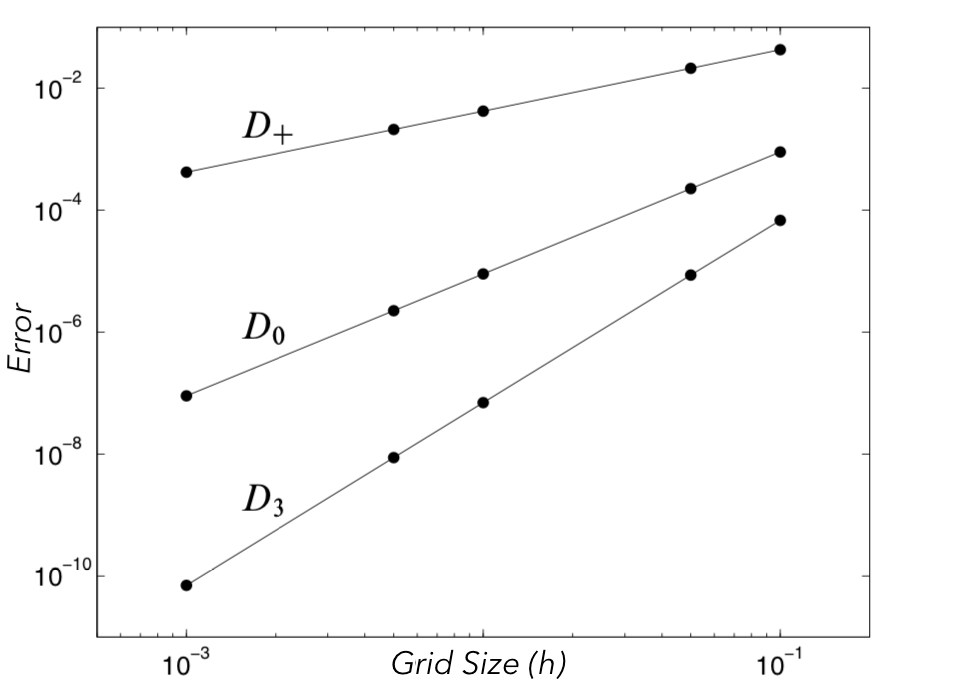
\includegraphics[width=0.5\textwidth]{leveque_errors_plotting}
	\caption{Plotting error for the different numerical differentiation schemes (plot extracted from reference \cite{leveque_ch1})}
\label{fig:leveque_errors_plotting}
\end{figure}

\newpage
\section{Applying Finite Difference Methods to PDEs}

For one dimensional diffusion-like equations

\begin{align}
\label{eq:generic-pde}
\frac{\partial f}{\partial t} &= \frac{\partial^2 f}{\partial x^2} + F(x, f(x), f'(x)).
\end{align}

We will discretize the derivative as described in \ref{eq:forward-difference} and replacing 

\begin{align}
	f(t_n, x_k) = \rho^{n,k},
\end{align}

which yields the following derivation rules for temporal and spacial derivatives
\begin{align}
\frac{\partial f}{\partial t} = \frac{\rho^{n+1, k}-\rho^{n, k}}{\Delta t},\\
\frac{\partial^2 f}{\partial x^2} = \frac{\rho^{n+1, k-1}-2\rho^{n, k}+\rho^{n+1, k+1}}{\Delta \xi^2}.
\end{align}

Replacing these approximations into equation \ref{eq:generic-pde} we get

\begin{align}	
\label{eq:linear-eq-numeric}
    -\alpha \rho^{n+1,k-1} + ( 1 + 2\alpha ) \rho^{n+1,k} -\alpha \rho^{n+1,k+1} =  \rho^{n,k}\\
    k \in [1, ... , m-1]
\end{align}

where $\alpha = \Delta t / \Delta x^2$.

\subsection{Boundary Conditions}

A reasonable question emerges when we are trying to solve the set of linear equations \ref{eq:linear-eq-numeric}: what happens with the equations at $k=1$ and $k=2$? Writing the explicitly
\begin{align}
    -\alpha \rho^{n+1,0} + ( 1 + \alpha ) \rho^{n+1,1} -\alpha \rho^{n+1,2} = \rho^{n,1},\\
    -\alpha \rho^{n+1,m-2} + ( 1 + 2\alpha ) \rho^{n+1,m-1} -\alpha \rho^{n+1,m} = \rho^{n,m-1},
    \label{eq:boundary-equations1}
\end{align}

from where we can recognize that we do not know the values of $\rho^{n+1,0}$ and $\rho^{n+1,m}$.

Boundary conditions (at least to the extent considered in this work) are of four types:

\begin{enumerate}
	\item Neumann boundary conditions: $f'(a) = \alpha$, $f'(b) = \beta$,
	\item Dirichlet boundary conditions: $f(a) = \alpha$, $f(b) = \beta$,
	\item Cauchy boundary conditions: $f(a) = \alpha$, $f'(b) = \beta$, or $f'(a) = \alpha$, $f(b) = \beta$,
	\item Robin boundary conditions: $\qty{w_1f'(x) + w_2f(x)}\big|_{\partial\Omega} = g$ , where $\partial\Omega$ is the boundary of the system.
\end{enumerate}

Particularely for the effect of this work we are interested in Cauchy and Robin boundary conditions. Each type of boundary condition deserves careful analysis.

\subsection{Cauchy boundary conditions}
Consider for the sake of the argument that we have Cauchy boundary conditions where 
\begin{align}
	\rho(t,0) = a,\\
	\rho(t,\delta) = b.
\end{align}

Then in discrete form 

\begin{align}
    \rho^{n, 0} = a + \rho^{n, 1}, \\
    \rho^{n, m-1} = b.
\end{align}

The boundary equations \ref{eq:boundary-equations1} thus yield

\begin{align}
	\label{eq:boundary-equations-cauchy}
    -\alpha \qty{a + \rho^{n+1, 1}}  + ( 1 + 2\alpha ) \rho^{n+1,1} -\alpha \rho^{n+1,2} = \rho^{n,1},\\
    -\alpha \rho^{n+1,m-2} + ( 1 + 2\alpha ) \rho^{n+1,m-1} - \alpha b = \rho^{n,m-1}.
\end{align}

We want to put these equations (the boundary equations and all the equations in between) in matrix form. Let 

\begin{align}
    \bf{\rho^n} = \begin{bmatrix}
                    \rho^{n, 1} \\
                    \vdots \\
                    \rho^{n, m-1} 
                    \end{bmatrix},
\end{align}

Since we need to include boundary conditions, we use equations \ref{eq:boundary-equations-cauchy} to eliminate $\rho^{n, 0}$, $\rho^{n, m}$. We want to write equations \ref{eq:boundary-equations-cauchy} as

\begin{align}
    \bf{\underline{A}} \bf{\rho^{n+1}}  = \bf{\rho^n} + \bf{b},
\end{align}

where

\begin{align}
    \bf{b} = \begin{bmatrix}
                    \alpha a \\
                    \vdots \\
                    0 \\
                    \alpha b 
                    \end{bmatrix},
\end{align}


and 

\begin{align}
\bf{\underline{A}} &= \begin{bmatrix}
           ( 1 + \alpha) & -\alpha  &  0 & 0 &  \cdots & 0\\
             -\alpha & ( 1 + 2 \alpha ) & -\alpha & \cdots & 0 & 0\\
           \vdots  &\cdots  & \ddots & \ddots &  \ddots&  \\
            \vdots & \cdots & 0  &  -\alpha & ( 1 + 2 \alpha ) & -\alpha \\
            0 & \cdots &0  & 0 & -\alpha & ( 1 + 2 \alpha )
         \end{bmatrix},
\end{align}

be an $m\times m$ matrix.

If the initial state of the system is $f(0,x)$, we get

\begin{align}
    \bf{\rho^{0,k}} = f(0, x_k), \\
    k \in [1,..., M-1].
\end{align}

This means that the dimensions of $\bf{\underline{A}}$ is $M-2 \times M-2$ and the numerical solution is solved in the interval  $k \in [0,..., M]$, leaving $k=0$ and $k=M$ as the overflow terms to push the boundary conditions.




\subsection{Robin boundary conditions}

Now we turn to the more complex case of Robin boundary conditions. We consider for simplicity the case of Robin boundary conditions at $x=0$ and Dirichlet boundary conditions at $x = \delta$. That is
\begin{align}
	\qty{w_1\frac{\partial \rho(t,0)}{\partial x}+w_2\rho(t,0)} = g,\\
	\rho(t,\delta) = b.
\end{align}

Then in discrete form 

\begin{align}
    w_1\frac{\rho^{n, 1}-\rho^{n,0}}{\Delta x} = a - w_2\rho^{n, 0}, \\
    \rho^{n, m-1} = b.
\end{align}

Therefore we can write

\begin{align}
	\rho^{n,1} = \frac{\Delta x a }{w_1} + \qty{1 - \frac{\Delta x w_2 }{w_1}}\rho^{n, 0}\\
\end{align}

\begin{align}
	\rho^{n, 0} = \frac{\rho^{n,1} - \frac{\Delta x a }{w_1}}{\qty{1 - \frac{\Delta x w_2 }{w_1}}} = \gamma\qty{\rho^{n,1} - \frac{\Delta x a }{w_1}} \\
\end{align}

Replacing this result in \ref{eq:boundary-equations-cauchy} 

\begin{align}
	\label{eq:boundary-equations-robin}
    -\alpha \gamma \qty{\rho^{n+1, 1} - \frac{\Delta x a }{w_1}}  + ( 1 + 2\alpha ) \rho^{n+1,1} -\alpha \rho^{n+1,2} = \rho^{n,1},\\
    -\alpha \rho^{n+1,m-2} + ( 1 + 2\alpha ) \rho^{n+1,m-1} - \alpha b = \rho^{n,m-1}.
\end{align}

As in the previous section, we want to write the $M$ equations as 

\begin{align}
    \bf{\underline{A}} \bf{\rho^{n+1}}  = \bf{\rho^n} + \bf{b}.
\end{align}

From equations \ref{eq:boundary-equations-robin} we get

\begin{align}
    \bf{b} = \begin{bmatrix}
                    -\frac{\Delta x a }{w_1}\alpha\gamma\\
                    \vdots \\
                    0 \\
                    \alpha b 
                    \end{bmatrix},
\end{align}


and 

\begin{align}
\bf{\underline{A}} &= \begin{bmatrix}
           ( 1 + 2\alpha-\gamma\alpha) & -\alpha  &  0 & 0 &  \cdots & 0\\
             -\alpha & ( 1 + 2 \alpha ) & -\alpha & \cdots & 0 & 0\\
           \vdots  &\cdots  & \ddots & \ddots &  \ddots&  \\
            \vdots & \cdots & 0  &  -\alpha & ( 1 + 2 \alpha ) & -\alpha \\
            0 & \cdots &0  & 0 & -\alpha & ( 1 + 2 \alpha )
         \end{bmatrix}
         \label{eq:discretization-matrix-with-bc},
\end{align}

be an $m\times m$ matrix. Where

\begin{align}
    \bf{\rho^{0,k}} = f(0, x_k). \\
\end{align}







